% Figura cuerpo B2: el modelo en el plano brecha-inflación: una perturbación de demanda no plantea disyuntiva; una de costes, sí
\documentclass[tikz,border=3pt]{standalone}
\usepackage[T1]{fontenc}
\usepackage[utf8]{inputenc}
\usepackage{amsmath}
\usetikzlibrary{arrows.meta,calc,positioning}
\begin{document}
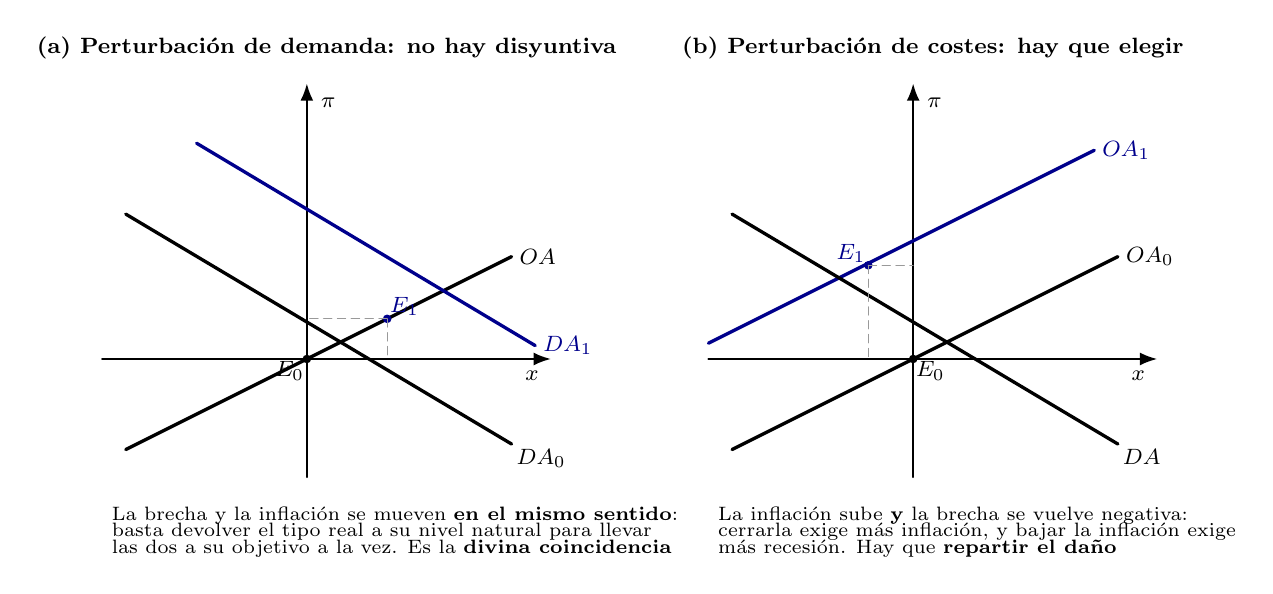
\begin{tikzpicture}[>={Latex[length=2.2mm]}, line cap=round, font=\footnotesize,
  eje/.style={->, thick},
  curva/.style={very thick},
  nueva/.style={very thick, blue!55!black},
  guia/.style={densely dashed, gray!80},
  pto/.style={circle, fill=black, inner sep=1.1pt}]
  % ---------- Panel (a): perturbacion de demanda ----------
  \node[font=\footnotesize\bfseries] at (0.25,3.95) {(a) Perturbación de demanda: no hay disyuntiva};
  \draw[eje] (-2.6,0) -- (3.1,0) node[below left=1pt]{$x$};
  \draw[eje] (0,-1.5) -- (0,3.5) node[below right=2pt]{$\pi$};
  % Oferta (PHILLIPS): pendiente positiva
  \draw[curva] (-2.3,-1.15) -- (2.6,1.3) node[right=-1pt]{$OA$};
  % Demanda (IS + regla): pendiente negativa
  \draw[curva] (-2.3,1.84) -- (2.6,-1.08) node[below right=-3pt]{$DA_0$};
  \draw[nueva] (-1.4,2.74) -- (2.9,0.17) node[right=-1pt]{$DA_1$};
  \node[pto] (E0) at (0,0) {};
  \node[below left=-2pt of E0, inner sep=1pt] {$E_0$};
  \node[pto, fill=blue!55!black] (E1) at (1.02,0.51) {};
  \node[above right=-2pt of E1, inner sep=1pt, blue!55!black] {$E_1$};
  \draw[guia] (1.02,0.51) -- (1.02,0);
  \draw[guia] (1.02,0.51) -- (0,0.51);
  \node[align=left, anchor=north west, font=\scriptsize] at (-2.6,-1.75)
    {La brecha y la inflación se mueven \textbf{en el mismo sentido}:\\[-2pt]basta devolver el tipo real a su nivel natural para llevar\\[-2pt]las dos a su objetivo a la vez. Es la \textbf{divina coincidencia}};
  % ---------- Panel (b): perturbacion de costes ----------
  \begin{scope}[xshift=7.7cm]
    \node[font=\footnotesize\bfseries] at (0.25,3.95) {(b) Perturbación de costes: hay que elegir};
    \draw[eje] (-2.6,0) -- (3.1,0) node[below left=1pt]{$x$};
    \draw[eje] (0,-1.5) -- (0,3.5) node[below right=2pt]{$\pi$};
    \draw[curva] (-2.3,-1.15) -- (2.6,1.3) node[right=-1pt]{$OA_0$};
    \draw[nueva] (-2.6,0.2) -- (2.3,2.65) node[right=-1pt]{$OA_1$};
    \draw[curva] (-2.3,1.84) -- (2.6,-1.08) node[below right=-3pt]{$DA$};
    \node[pto] (F0) at (0,0) {};
    \node[below right=-2pt of F0, inner sep=1pt] {$E_0$};
    \node[pto, fill=blue!55!black] (F1) at (-0.57,1.19) {};
    \node[above left=-2pt of F1, inner sep=1pt, blue!55!black] {$E_1$};
    \draw[guia] (-0.57,1.19) -- (-0.57,0);
    \draw[guia] (-0.57,1.19) -- (0,1.19);
    \node[align=left, anchor=north west, font=\scriptsize] at (-2.6,-1.75)
      {La inflación sube \textbf{y} la brecha se vuelve negativa:\\[-2pt]cerrarla exige más inflación, y bajar la inflación exige\\[-2pt]más recesión. Hay que \textbf{repartir el daño}};
  \end{scope}
\end{tikzpicture}
\end{document}
